\section[Algorithmen]{Algorithmen}
\label{sec:Algorithmen}
Die für einen Jouney Planner zu lösende Aufgabe ist das Shortest-Path Problem. Un dieses Problem zu lösen, gibt es mehrere Herangehensweisen. 

\subsection{Graph Basierte Algorithmen}
\label{sec:Graph Basierte Algorithmen}
Graph-Basierte Algorithmen bilden einen Graphen aus Punkten. Die Verbindungen zwischen den Punkten werden mit einer Gewichtung versehen. Der Algorithmus iteriert nun über den Graphen und findet die Verbindung zwischen dem Start- und Endpunkt mit dem niedrigsten kombinierten Gewicht.

\subsubsection{Dijkstra}
\label{sec:Dijkstra}
Der Dijkstra Algorithmus ist ein Single-Source-Shortest-Path Algorithmus. Er berechnet den kürzesten Weg von einem Startnode zu jedem anderen \gls{Node} im Graphen. Er iteriert über alle möglichen Verbindungen und speichert das Gewicht eines Zielnodes. Wenn eine weitere Verbindung zum gleichen Node gefunden wird, so wird die Verbindung mit dem geringsten Gewicht behalten. Es wird immer die Node mit dem geringsten Gewichtswert zum Startnode als nächstes berechnet. Wenn auch der Zielnode bekannt ist, wird der Algorithmus gleichzeitig vom Start und Zielnode aus gestartet, so dass sie sich in der Mitte treffen. 

Der Dijkstra Algorithmus ist der Basisalgorithmus mit dem die anderen Algorithmen verglichen werden. Er ist konzeptionell einfach, jedoch in keiner Weise optimiert. Die Laufzeit erhöht sich exponentiell mit der Anzahl der Nodes und Verbindungen, weshalb er für grosse Netzwerke ungeeignet ist. ~\cite{dij_a} ~\cite{dij_bell}

\subsubsection{A*}
\label{sec:A*}
Der A* Algorithmus ist eine Erweiterung des Dijkstar Algorithmus. Er sucht nicht wie der Dijkstra Algorithmus linear in alle Richtungen, sondern gezielt in Richtung des Zielnodes. Dazu wird jedem Punkt im Graph eine Entfernung zum Zielnodes zugewiesen. Nun wird dieser Wert mit dem Gewichtswert des Abstandes zum Startnode kombiniert. Der als nächstes zu berechnende Punkt wird nun aufgrund dieses Wertes entschieden. Dadurch werden Verbindungen welche in Richtung des Zieles führen präferiert und es werden viele überflüssige Rechenschritte eingespart.

Obwohl der A* Algorithmus mehr Operationen pro Node durchführen muss, hat er dennoch eine höhere Performance als der Dijkstra Algorithmus, da viel weniger Nodes untersucht werden müssen. Der Nachteil vom A* Algorithmus ist, dass er mehr Memory benötigt. ~\cite{dij_a}

 

\subsubsection{Bellman-Ford}
\label{sec:Bellman-Ford}
Der Bellman-Ford Algorithmus verwendet das gleiche Grundkonzept wie der Dijkstra Algorithmus. Er achtet jedoch nicht auf den geringsten Gewichtungsfaktor zum Startnode, sondern geht der Reihe nach alle Nodes durch. Wenn nun für einen Node nicht alle Zwischennodes zum Starnode schon berechnet wurden, so scheint dieser Node unerreichbar. Um diese Problematik zu lösen wird dieser Prozess x-1 mal wiederholt, wobei x die Anzahl der Nodes ist. ~\cite{dij_bell} ~\cite{bell}

Der Bellman-Ford Algorithmus ist langsamer als der Dijkstra Algorithmus, da er mehrere Durchläufe über alle Nodes benötigt. Dies bietet ihm jedoch den Vorteil, dass auch eine negative Gewichtung einer Verbindung möglich ist.

\subsection{Non Graph Basierte Algorithmen}
\label{sec:Non Graph Basierte Algorithmen}
In diesem Abschnitt werden Algorithmen erläutert, welche nicht auf das Grundkonzept des Dijkstra Algorithmus aufbauen.

\subsubsection{RAPTOR}
\label{sec:RAPTOR}
Der Round-Based Public Transit Routing Algorithmus, auch RAPTOR Algorithmus genannt, ist ein Rundenbasierter, auf öffentliche Verkehrsnetzwerke zugeschnittener Algorithmus, welcher auf die vorgegebenen Zuglinien achtet.

Der RAPTOR Algorithmus durchläuft mehrere Runden um von der Startstation zur Zielstation zu finden. In der ersten Runde werden alle Zuglinien gescannt, welche durch die Startstation verlaufen. Wenn eine andere Zuglinie die gescannte Zuglinie kreuzt, so wird die andere Zuglinie sowie die Kreuzungsstation markiert. In der nächsten Runde werden nun alle markierten Zuglinien gescannt. Dieser Prozess wird so lange weitergeführt, bis sich die Zielstation in einer gescannten Zuglinie befindet. Nun kann anhand der Kreuzungsstationen die Route erstellt werden.

Der RAPTOR Algorithmus besitzt eine höhere Performanz als alle Graph Basierten Algorithmen. ~\cite{raptor}

\subsubsection{Connection Scan Algorithm}
\label{sec:Connection Scan Algorithm}
Der Connection Scan Algorithm, kurz CSA, ist schon vom Grundkonzept her auf Zeitplanbasierte Netzwerke zugeschnitten. Er arbeitet mit Stations\gls{stations}, Connections\gls{connections}, Trips\gls{trips} und Footpaths\gls{footpaths}. 

In einem Ersten Schritt werden die Daten in die benötigte Timetable-Form gebracht und alle Connections nach der Abfahrtszeit sortiert. Diese Schritte werden preprocessed. Danach wird über alle Connections iteriert. Eine Connection wird als erreichbar markiert, wenn sie an bereits als erreichbar markierte Connections anschliesst oder mit der Startstation verbunden ist. Dies wird dann solange durchgeführt, bis die Zielstation erreicht ist. Anschliessend wird von der Zielstation aus der verfolgte Weg zusammengesetzt, so dass ein Journey von der Startstation zur Zielstation entsteht. 

Für grosse Netzwerke kann der CSA mit einem Quadtree-Preprocessing Schritt erweitert werden. Dabei wird das Netzwerk in immer kleiner werdende Quadrate unterteilt. Für Quadrate welche nicht die Start- oder Zielstation enthalten, müssen nun nur noch die Connections beachtet werden, welche über die Ränder des Quadrates hinaus gehen. Somit können für Fernverbindungen die lokalen Connections ignoriert werden.
\begin{figure}[]
	\centering
	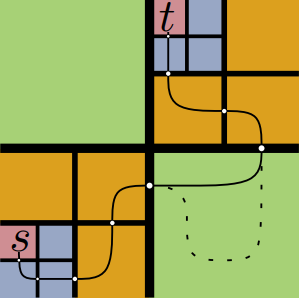
\includegraphics[width=8cm]{QuadTree.png}
	\caption{Veranschaulichung der Funktion des QuadTree-Preprocessings ~\cite{csa}}
	\label{fig:QuadTree}
\end{figure}


Im Gegensatz zum Dijkstra müssen beim CSA die Connections nicht nach dem nächsten Schritt durchsucht werden, da die Abfolge durch die Preprocessing-Schritte schon definiert wurde. Dies führt zu einer Performanceverbesserung im mehrstelligen Bereich. Ein Nachteil ist jedoch, dass Preprocessing-Schritte von Nöten sind und so nicht in echtzeit auf Verspätungen reagiert werden kann. Da diese Schritte jedoch nur wenige Sekunden benötigen ist dies kein schwerwiegender Nachteil. Mit der Erweiterung des Quadtree-Preprocessings können auch Anfragen in landesweite Netzwerke in wenigen Millisekunden berechnet werden. 

Im Vergleich zum RAPTOR Algorithmus bietet der CSA eine höhere Performance. ~\cite{csa}


\subsection{Transfer Pattern}
\label{sec:Transfer Pattern}
Transfer Pattern ist eine Algorithmusstrategie welche auf Preprocessing setzt. Alle möglichen Verbindungen werden mithilfe eines Algorithmuses berechnet und in einem Datensatz gespeichert. Die eigentliche Anfrage beschränkt sich dann auf eine Query-Abfrage auf diesen Datensatz.

Für das Preprocessing können alle zuvor genannten Algorithmen verwendet werden. Die Dijksta basierten Algorithen haben jedoch den Nachteil, dass Query anfragen für landesweite Netzwerke immer noch mehrere Sekunden benötigen, weshalb der RAPTOR Algorithmus oder der CSA zu bevorzugen sind. ~\cite{transferpatterns_alenex}

Um das Preprocessing zu beschleunigen können mehrere Erweiterungen hinzugefügt werden. Eine davon ist die Verwendung von Hubs. Dabei werden die grössten Stationen als Hubs markiert. Zwischen diesen Hubs werden alle Transfer Pattern berechnet. Bei Stationen welche keine Hubs sind werden nur die Verbindungen bis zum nächsten Hub berechnet. Sollte nach drei Zugwechseln kein Hub erreicht sein so wird die Verbindung verworfen. Dies kann zwar zu Fehlern führen, ist aber vernachlässigbar, da die Fehlerrate laut Experimenten bei drei Promille liegt. ~\cite{transferpatterns_esa}

Der Preprocessing\gls{preprocessing} kann je nach Grösse und Struktur des Netzwerks eine lange Zeit in Anspruch nehmen. Selbst mit allen Erweiterungen braucht das Preprocessing für das CH-Netzwerk vier Stunden. Dafür benötigen die Query-Anfragen nur wenige Millisekunden. Der Nachteil ist jedoch, dass mit Transfer Pattern nicht auf Zugverspätungen und Fahrplanänderungen reagiert werden kann. 





